\section*{Задание 4}

\subsection*{Задание}

Постройте код Прюфера для данного дерева

\begin{figure}[H]
    \centering
    \begin{tikzpicture}[>=latex,line join=bevel,]
        %%
        \node (3) at (45.0bp,306.0bp) [draw,rectangle] {3};
        \node (4) at (45.0bp,234.0bp) [draw,rectangle] {4};
        \node (5) at (45.0bp,162.0bp) [draw,rectangle] {5};
        \node (6) at (27.0bp,90.0bp) [draw,rectangle] {6};
        \node (10) at (99.0bp,90.0bp) [draw,rectangle] {10};
        \node (1) at (243.0bp,162.0bp) [draw,rectangle] {1};
        \node (7) at (243.0bp,90.0bp) [draw,rectangle] {7};
        \node (8) at (315.0bp,90.0bp) [draw,rectangle] {8};
        \node (9) at (171.0bp,90.0bp) [draw,rectangle] {9};
        \node (2) at (153.0bp,162.0bp) [draw,rectangle] {2};
        \node (11) at (99.0bp,18.0bp) [draw,rectangle] {11};
        \draw [] (3) ..controls (45.0bp,276.85bp) and (45.0bp,262.92bp)  .. (4);
        \draw [] (4) ..controls (45.0bp,204.85bp) and (45.0bp,190.92bp)  .. (5);
        \draw [] (5) ..controls (37.76bp,132.85bp) and (34.179bp,118.92bp)  .. (6);
        \draw [] (5) ..controls (66.719bp,132.85bp) and (77.464bp,118.92bp)  .. (10);
        \draw [] (1) ..controls (243.0bp,132.85bp) and (243.0bp,118.92bp)  .. (7);
        \draw [] (1) ..controls (271.96bp,132.85bp) and (286.29bp,118.92bp)  .. (8);
        \draw [] (1) ..controls (214.04bp,132.85bp) and (199.71bp,118.92bp)  .. (9);
        \draw [] (2) ..controls (160.24bp,132.85bp) and (163.82bp,118.92bp)  .. (9);
        \draw [] (2) ..controls (131.28bp,132.85bp) and (120.54bp,118.92bp)  .. (10);
        \draw [] (10) ..controls (99.0bp,60.846bp) and (99.0bp,46.917bp)  .. (11);
        %
    \end{tikzpicture}
    \caption{}
\end{figure}

\subsection*{Решение}

Допустим корнем дерева будет вершина с номером \textbf{5}.
Тогда:

\textbf{Шаг 1}

Граф:

\begin{tikzpicture}[>=latex,line join=bevel,]
    %%
    \node (3) at (45.0bp,306.0bp) [draw=red,rectangle] {3};
    \node (4) at (45.0bp,234.0bp) [draw=green,rectangle] {4};
    \node (5) at (45.0bp,162.0bp) [draw=blue,rectangle] {5};
    \node (6) at (27.0bp,90.0bp) [draw,rectangle] {6};
    \node (10) at (99.0bp,90.0bp) [draw,rectangle] {10};
    \node (1) at (243.0bp,162.0bp) [draw,rectangle] {1};
    \node (7) at (243.0bp,90.0bp) [draw,rectangle] {7};
    \node (8) at (315.0bp,90.0bp) [draw,rectangle] {8};
    \node (9) at (171.0bp,90.0bp) [draw,rectangle] {9};
    \node (2) at (153.0bp,162.0bp) [draw,rectangle] {2};
    \node (11) at (99.0bp,18.0bp) [draw,rectangle] {11};
    \draw [] (3) ..controls (45.0bp,276.85bp) and (45.0bp,262.92bp)  .. (4);
    \draw [] (4) ..controls (45.0bp,204.85bp) and (45.0bp,190.92bp)  .. (5);
    \draw [] (5) ..controls (37.76bp,132.85bp) and (34.179bp,118.92bp)  .. (6);
    \draw [] (5) ..controls (66.719bp,132.85bp) and (77.464bp,118.92bp)  .. (10);
    \draw [] (1) ..controls (243.0bp,132.85bp) and (243.0bp,118.92bp)  .. (7);
    \draw [] (1) ..controls (271.96bp,132.85bp) and (286.29bp,118.92bp)  .. (8);
    \draw [] (1) ..controls (214.04bp,132.85bp) and (199.71bp,118.92bp)  .. (9);
    \draw [] (2) ..controls (160.24bp,132.85bp) and (163.82bp,118.92bp)  .. (9);
    \draw [] (2) ..controls (131.28bp,132.85bp) and (120.54bp,118.92bp)  .. (10);
    \draw [] (10) ..controls (99.0bp,60.846bp) and (99.0bp,46.917bp)  .. (11);
    %
\end{tikzpicture}

Лист дерева с минимальным номером: 3

Добавляем номер родителя минимального листа в код и убираем минимальный лист из графа.

Код: 4

\textbf{Шаг 2}

Граф:

\begin{tikzpicture}[>=latex,line join=bevel,]
    %%
    \node (4) at (45.0bp,234.0bp) [draw=red,rectangle] {4};
    \node (5) at (45.0bp,162.0bp) [draw=green,rectangle] {5};
    \node (6) at (27.0bp,90.0bp) [draw,rectangle] {6};
    \node (10) at (99.0bp,90.0bp) [draw,rectangle] {10};
    \node (1) at (243.0bp,162.0bp) [draw,rectangle] {1};
    \node (7) at (243.0bp,90.0bp) [draw,rectangle] {7};
    \node (8) at (315.0bp,90.0bp) [draw,rectangle] {8};
    \node (9) at (171.0bp,90.0bp) [draw,rectangle] {9};
    \node (2) at (153.0bp,162.0bp) [draw,rectangle] {2};
    \node (11) at (99.0bp,18.0bp) [draw,rectangle] {11};
    \draw [] (4) ..controls (45.0bp,204.85bp) and (45.0bp,190.92bp)  .. (5);
    \draw [] (5) ..controls (37.76bp,132.85bp) and (34.179bp,118.92bp)  .. (6);
    \draw [] (5) ..controls (66.719bp,132.85bp) and (77.464bp,118.92bp)  .. (10);
    \draw [] (1) ..controls (243.0bp,132.85bp) and (243.0bp,118.92bp)  .. (7);
    \draw [] (1) ..controls (271.96bp,132.85bp) and (286.29bp,118.92bp)  .. (8);
    \draw [] (1) ..controls (214.04bp,132.85bp) and (199.71bp,118.92bp)  .. (9);
    \draw [] (2) ..controls (160.24bp,132.85bp) and (163.82bp,118.92bp)  .. (9);
    \draw [] (2) ..controls (131.28bp,132.85bp) and (120.54bp,118.92bp)  .. (10);
    \draw [] (10) ..controls (99.0bp,60.846bp) and (99.0bp,46.917bp)  .. (11);
    %
\end{tikzpicture}

Лист дерева с минимальным номером: 4

Добавляем номер родителя минимального листа в код и убираем минимальный лист из графа.

Код: 4, 5

\textbf{Шаг 3}

Граф:

\begin{tikzpicture}[>=latex,line join=bevel,]
    %%
    \node (5) at (45.0bp,162.0bp) [draw=green,rectangle] {5};
    \node (6) at (27.0bp,90.0bp) [draw=red,rectangle] {6};
    \node (10) at (99.0bp,90.0bp) [draw,rectangle] {10};
    \node (1) at (243.0bp,162.0bp) [draw,rectangle] {1};
    \node (7) at (243.0bp,90.0bp) [draw,rectangle] {7};
    \node (8) at (315.0bp,90.0bp) [draw,rectangle] {8};
    \node (9) at (171.0bp,90.0bp) [draw,rectangle] {9};
    \node (2) at (153.0bp,162.0bp) [draw,rectangle] {2};
    \node (11) at (99.0bp,18.0bp) [draw,rectangle] {11};
    \draw [] (5) ..controls (37.76bp,132.85bp) and (34.179bp,118.92bp)  .. (6);
    \draw [] (5) ..controls (66.719bp,132.85bp) and (77.464bp,118.92bp)  .. (10);
    \draw [] (1) ..controls (243.0bp,132.85bp) and (243.0bp,118.92bp)  .. (7);
    \draw [] (1) ..controls (271.96bp,132.85bp) and (286.29bp,118.92bp)  .. (8);
    \draw [] (1) ..controls (214.04bp,132.85bp) and (199.71bp,118.92bp)  .. (9);
    \draw [] (2) ..controls (160.24bp,132.85bp) and (163.82bp,118.92bp)  .. (9);
    \draw [] (2) ..controls (131.28bp,132.85bp) and (120.54bp,118.92bp)  .. (10);
    \draw [] (10) ..controls (99.0bp,60.846bp) and (99.0bp,46.917bp)  .. (11);
    %
\end{tikzpicture}

Лист дерева с минимальным номером: 6

Добавляем номер родителя минимального листа в код и убираем минимальный лист из графа.

Код: 4, 5, 5

\textbf{Шаг 4}

Граф:

\begin{tikzpicture}[>=latex,line join=bevel,]
    %%
    \node (5) at (27.0bp,162.0bp) [draw=black,rectangle] {5};
    \node (10) at (27.0bp,90.0bp) [draw,rectangle] {10};
    \node (1) at (171.0bp,162.0bp) [draw=green,rectangle] {1};
    \node (7) at (171.0bp,90.0bp) [draw=red,rectangle] {7};
    \node (8) at (243.0bp,90.0bp) [draw,rectangle] {8};
    \node (9) at (99.0bp,90.0bp) [draw,rectangle] {9};
    \node (2) at (99.0bp,162.0bp) [draw,rectangle] {2};
    \node (11) at (27.0bp,18.0bp) [draw,rectangle] {11};
    \draw [] (5) ..controls (27.0bp,132.85bp) and (27.0bp,118.92bp)  .. (10);
    \draw [] (1) ..controls (171.0bp,132.85bp) and (171.0bp,118.92bp)  .. (7);
    \draw [] (1) ..controls (199.96bp,132.85bp) and (214.29bp,118.92bp)  .. (8);
    \draw [] (1) ..controls (142.04bp,132.85bp) and (127.71bp,118.92bp)  .. (9);
    \draw [] (2) ..controls (99.0bp,132.85bp) and (99.0bp,118.92bp)  .. (9);
    \draw [] (2) ..controls (70.042bp,132.85bp) and (55.714bp,118.92bp)  .. (10);
    \draw [] (10) ..controls (27.0bp,60.846bp) and (27.0bp,46.917bp)  .. (11);
    %
\end{tikzpicture}

Лист дерева с минимальным номером: 7

Добавляем номер родителя минимального листа в код и убираем минимальный лист из графа.

Код: 4, 5, 5, 1

\textbf{Шаг 5}

Граф:

\begin{tikzpicture}[>=latex,line join=bevel,]
    %%
    \node (5) at (27.0bp,162.0bp) [draw=black,rectangle] {5};
    \node (10) at (27.0bp,90.0bp) [draw,rectangle] {10};
    \node (1) at (171.0bp,162.0bp) [draw=green,rectangle] {1};
    \node (8) at (171.0bp,90.0bp) [draw=red,rectangle] {8};
    \node (9) at (99.0bp,90.0bp) [draw,rectangle] {9};
    \node (2) at (99.0bp,162.0bp) [draw,rectangle] {2};
    \node (11) at (27.0bp,18.0bp) [draw,rectangle] {11};
    \draw [] (5) ..controls (27.0bp,132.85bp) and (27.0bp,118.92bp)  .. (10);
    \draw [] (1) ..controls (171.0bp,132.85bp) and (171.0bp,118.92bp)  .. (8);
    \draw [] (1) ..controls (142.04bp,132.85bp) and (127.71bp,118.92bp)  .. (9);
    \draw [] (2) ..controls (99.0bp,132.85bp) and (99.0bp,118.92bp)  .. (9);
    \draw [] (2) ..controls (70.042bp,132.85bp) and (55.714bp,118.92bp)  .. (10);
    \draw [] (10) ..controls (27.0bp,60.846bp) and (27.0bp,46.917bp)  .. (11);
    %
\end{tikzpicture}

Лист дерева с минимальным номером: 8

Добавляем номер родителя минимального листа в код и убираем минимальный лист из графа.

Код: 4, 5, 5, 1, 1

\textbf{Шаг 6}

Граф:

\begin{tikzpicture}[>=latex,line join=bevel,]
    %%
    \node (5) at (27.0bp,162.0bp) [draw=black,rectangle] {5};
    \node (10) at (45.0bp,90.0bp) [draw,rectangle] {10};
    \node (1) at (171.0bp,162.0bp) [draw=red,rectangle] {1};
    \node (9) at (153.0bp,90.0bp) [draw=green,rectangle] {9};
    \node (2) at (99.0bp,162.0bp) [draw,rectangle] {2};
    \node (11) at (45.0bp,18.0bp) [draw,rectangle] {11};
    \draw [] (5) ..controls (34.24bp,132.85bp) and (37.821bp,118.92bp)  .. (10);
    \draw [] (1) ..controls (163.76bp,132.85bp) and (160.18bp,118.92bp)  .. (9);
    \draw [] (2) ..controls (120.72bp,132.85bp) and (131.46bp,118.92bp)  .. (9);
    \draw [] (2) ..controls (77.281bp,132.85bp) and (66.536bp,118.92bp)  .. (10);
    \draw [] (10) ..controls (45.0bp,60.846bp) and (45.0bp,46.917bp)  .. (11);
    %
\end{tikzpicture}

Лист дерева с минимальным номером: 1

Добавляем номер родителя минимального листа в код и убираем минимальный лист из графа.

Код: 4, 5, 5, 1, 1, 9

\textbf{Шаг 7}

Граф:

\begin{tikzpicture}[>=latex,line join=bevel,]
    %%
    \node (5) at (27.0bp,162.0bp) [draw=black,rectangle] {5};
    \node (10) at (27.0bp,90.0bp) [draw,rectangle] {10};
    \node (9) at (99.0bp,90.0bp) [draw=red,rectangle] {9};
    \node (2) at (99.0bp,162.0bp) [draw=green,rectangle] {2};
    \node (11) at (27.0bp,18.0bp) [draw,rectangle] {11};
    \draw [] (5) ..controls (27.0bp,132.85bp) and (27.0bp,118.92bp)  .. (10);
    \draw [] (2) ..controls (99.0bp,132.85bp) and (99.0bp,118.92bp)  .. (9);
    \draw [] (2) ..controls (70.042bp,132.85bp) and (55.714bp,118.92bp)  .. (10);
    \draw [] (10) ..controls (27.0bp,60.846bp) and (27.0bp,46.917bp)  .. (11);
    %
\end{tikzpicture}

Лист дерева с минимальным номером: 9

Добавляем номер родителя минимального листа в код и убираем минимальный лист из графа.

Код: 4, 5, 5, 1, 1, 9, 2

\textbf{Шаг 8}

Граф:

\begin{tikzpicture}[>=latex,line join=bevel,]
    %%
    \node (5) at (27.0bp,162.0bp) [draw=black,rectangle] {5};
    \node (10) at (63.0bp,90.0bp) [draw=green,rectangle] {10};
    \node (2) at (99.0bp,162.0bp) [draw=red,rectangle] {2};
    \node (11) at (63.0bp,18.0bp) [draw,rectangle] {11};
    \draw [] (5) ..controls (41.479bp,132.85bp) and (48.643bp,118.92bp)  .. (10);
    \draw [] (2) ..controls (84.521bp,132.85bp) and (77.357bp,118.92bp)  .. (10);
    \draw [] (10) ..controls (63.0bp,60.846bp) and (63.0bp,46.917bp)  .. (11);
    %
\end{tikzpicture}

Лист дерева с минимальным номером: 2

Добавляем номер родителя минимального листа в код и убираем минимальный лист из графа.

Код: 4, 5, 5, 1, 1, 9, 2, 10

\textbf{Шаг 9}

Граф:

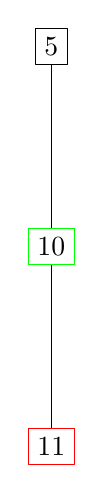
\begin{tikzpicture}[>=latex,line join=bevel,]
    %%
    \node (5) at (27.0bp,162.0bp) [draw=black,rectangle] {5};
    \node (10) at (27.0bp,90.0bp) [draw=green,rectangle] {10};
    \node (11) at (27.0bp,18.0bp) [draw=red,rectangle] {11};
    \draw [] (5) ..controls (27.0bp,132.85bp) and (27.0bp,118.92bp)  .. (10);
    \draw [] (10) ..controls (27.0bp,60.846bp) and (27.0bp,46.917bp)  .. (11);
    %
\end{tikzpicture}

Лист дерева с минимальным номером: 11

Добавляем номер родителя минимального листа в код и убираем минимальный лист из графа.

Код: 4, 5, 5, 1, 1, 9, 2, 10, 10

\textbf{Ответ}: 4, 5, 5, 1, 1, 9, 2, 10, 10